\newpage
\section{Data and Results}
\label{sec:data-results}

\subsection{Input data}

We set up three hits on the same satellite. The inputs are not measured
data; we chose values that are typical for a small Earth-observation
satellite and a millimetre-sized aluminium fragment.
Table~\ref{tab:inputs} shows the values that all scenarios share, and
Table~\ref{tab:scenarios} shows the ones that change. With
$\alpha=90^\circ$ the panel normal is $\hat{\vect n}=(0,1)$, the tangent
is $\hat{\vect t}=(-1,0)$ and the lever arm is $b=4\unit{m}$. From these
inputs the program also gets the fragment's diameter ($8.91\unit{mm}$),
its kinetic energy ($K_0=50\,000\unit{J}$) and the orbital speed
($v_{\mathrm{orb}}=7585.09\unit{m\,s^{-1}}$, Eq.~\eqref{eq:vorb}).

\begin{table}[H]
  \centering\footnotesize
  \caption{Input data shared by the three scenarios.}
  \label{tab:inputs}
  \begin{tabular}{@{}llr@{}}
    \toprule
    Quantity & Symbol & Value \\
    \midrule
    Satellite mass & $M$ & $500\unit{kg}$ \\
    Moment of inertia about the CoM & $I$ & $1200\unit{kg\,m^2}$ \\
    Impact point from the CoM & $\vect r$ & $(4,\,0)\unit{m}$ \\
    Panel normal direction from $+x$ & $\alpha$ & $90^\circ$ \\
    Debris mass and material & $m$ & $0.001\unit{kg}$, aluminium \\
    Debris density & $\rho$ & $2700\unit{kg\,m^{-3}}$ \\
    Relative impact speed & $v_0$ & $10\,000\unit{m\,s^{-1}}$ \\
    Orbit altitude & $h$ & $550\unit{km}$ \\
    Earth gravitational parameter & $\mu_E$ & $3.986004418\times10^{14}\unit{m^3\,s^{-2}}$ \\
    Earth radius & $R_E$ & $6\,378\,137\unit{m}$ \\
    \bottomrule
  \end{tabular}
\end{table}

\begin{table}[H]
  \centering\footnotesize
  \caption{Scenario-specific inputs.}
  \label{tab:scenarios}
  \begin{tabular}{@{}lll@{}}
    \toprule
    Scenario & Impact angle $\theta$ & Collision type \\
    \midrule
    Baseline & $30^\circ$ & completely inelastic (fragment embeds) \\
    Head-on embedding & $0^\circ$ & completely inelastic \\
    Grazing elastic & $80^\circ$ & elastic (fragment rebounds) \\
    \bottomrule
  \end{tabular}
\end{table}

\subsection{Scenario results}

Table~\ref{tab:results} shows the results. A negative $\omega$ means a
clockwise spin about $z$, which makes sense for a push in the $-y$
direction at $x=+4\unit{m}$. Velocities are measured in the frame that
moved with the satellite before the hit. The conservation errors from
Eq.~\eqref{eq:residuals} (last three rows) are all about $10^{-16}$, which
is just computer round-off. For example, $L_z=-34.641\unit{kg\,m^2\,s^{-1}}$
both before and after in the baseline, and $|\vect P|=10.000\unit{kg\,m\,s^{-1}}$
in all three scenarios.

\begin{table}[H]
  \centering\footnotesize
  \caption{Calculated results for the three scenarios.}
  \label{tab:results}
  \begin{tabular}{@{}lrrr@{}}
    \toprule
    Output quantity & Baseline & Head-on & Grazing \\
    \midrule
    Impulse on satellite $M|\Delta\vect V|$ (N\,s) & 9.99988 & 9.99985 & 3.47291 \\
    $|\Delta\vect V|$ (mm\,s$^{-1}$) & 19.9998 & 19.9997 & 6.94582 \\
    $\omega$ (rad\,s$^{-1}$) & $-0.0288671$ & $-0.0333328$ & $-0.0115764$ \\
    $|\omega|$ ($^\circ$\,s$^{-1}$) & 1.654 & 1.910 & 0.663 \\
    Fragment velocity after, $\vect v_{d1}$ (m\,s$^{-1}$) & $(0.0100,\,-0.133)$ & $(0,\,-0.153)$ & $(9848.08,\,1736.43)$ \\
    Fragment $K_{d1}$ (J) & $8.9\times10^{-6}$ & $1.2\times10^{-5}$ & 49\,999.908 \\
    Satellite $K_T$ (J) & 0.100 & 0.100 & 0.0121 \\
    Satellite $K_R$ (J) & 0.500 & 0.667 & 0.0804 \\
    $E_{\mathrm{diss}}$ (J) & 49\,999.400 & 49\,999.233 & 0 \\
    $E_{\mathrm{diss}}/K_0$ & 0.999988 & 0.999985 & 0 \\
    $|\Delta\vect V|/v_{\mathrm{orb}}$ & $2.64\times10^{-6}$ & $2.64\times10^{-6}$ & $9.16\times10^{-7}$ \\
    \midrule
    Residual $\varepsilon_P$ (Eq.~\eqref{eq:residuals}) & $8.9\times10^{-17}$ & 0 & 0 \\
    Residual $\varepsilon_L$ & $1.8\times10^{-16}$ & $3.6\times10^{-16}$ & 0 \\
    Residual $\varepsilon_E$ & 0 & 0 & $1.5\times10^{-16}$ \\
    \bottomrule
  \end{tabular}
\end{table}


\paragraph{Sample calculation (baseline, completely inelastic).}
From Eq.~\eqref{eq:vd0}, $\vect v_{d0}=(5000,\,-8660.25)\unit{m\,s^{-1}}$.
Equations~\eqref{eq:rc}--\eqref{eq:omega-inelastic} give
\begin{equation}
  \begin{aligned}
    \vect r_c &= \frac{(0.001)(4,0)}{500.001}=(8.0\times10^{-6},\,0)\unit{m},\qquad
    \vect v_{CM} = \frac{0.001\,\vect v_{d0}}{500.001}=(0.0100,\,-0.01732)\unit{m\,s^{-1}},\\
    I_c &= 1200 + 500(8.0\times10^{-6})^2 + 0.001(3.999992)^2 = 1200.016\unit{kg\,m^2},\\
    \omega &= \frac{0.001\,(3.999992)(-8660.25)}{1200.016} = -0.028867\unit{rad\,s^{-1}},\\
    E_{\mathrm{diss}} &= 50\,000 - \tfrac12(500.001)(0.02000)^2 - \tfrac12(1200.016)(0.028867)^2
      = 49\,999.40\unit{J}.
  \end{aligned}
  \label{eq:sample-inelastic}
\end{equation}
\paragraph{Sample calculation (grazing, elastic).}
$v_n=10\,000\cos80^\circ=1736.48\unit{m\,s^{-1}}$, $k=1000+0.002+16/1200=1000.0153\unit{kg^{-1}}$
(Eq.~\eqref{eq:k}), so $J=2(1736.48)/1000.0153=3.47291\unit{N\,s}$,
$|\Delta\vect V|=J/M=6.94582\unit{mm\,s^{-1}}$ and $\omega=-Jb/I=-0.0115764\unit{rad\,s^{-1}}$
(Eqs.~\eqref{eq:impulse}--\eqref{eq:J-elastic}).

Figure~\ref{fig:budget} shows where the momentum and energy go. In the
baseline, the satellite gets both the normal and the sideways momentum of
the fragment, and almost all of $K_0$ is lost. In the grazing elastic
case, only the normal momentum of the fragment is reversed, and the
fragment keeps almost all of its energy.

\begin{figure}[H]
  \centering
  \begin{subfigure}{\linewidth}\centering
    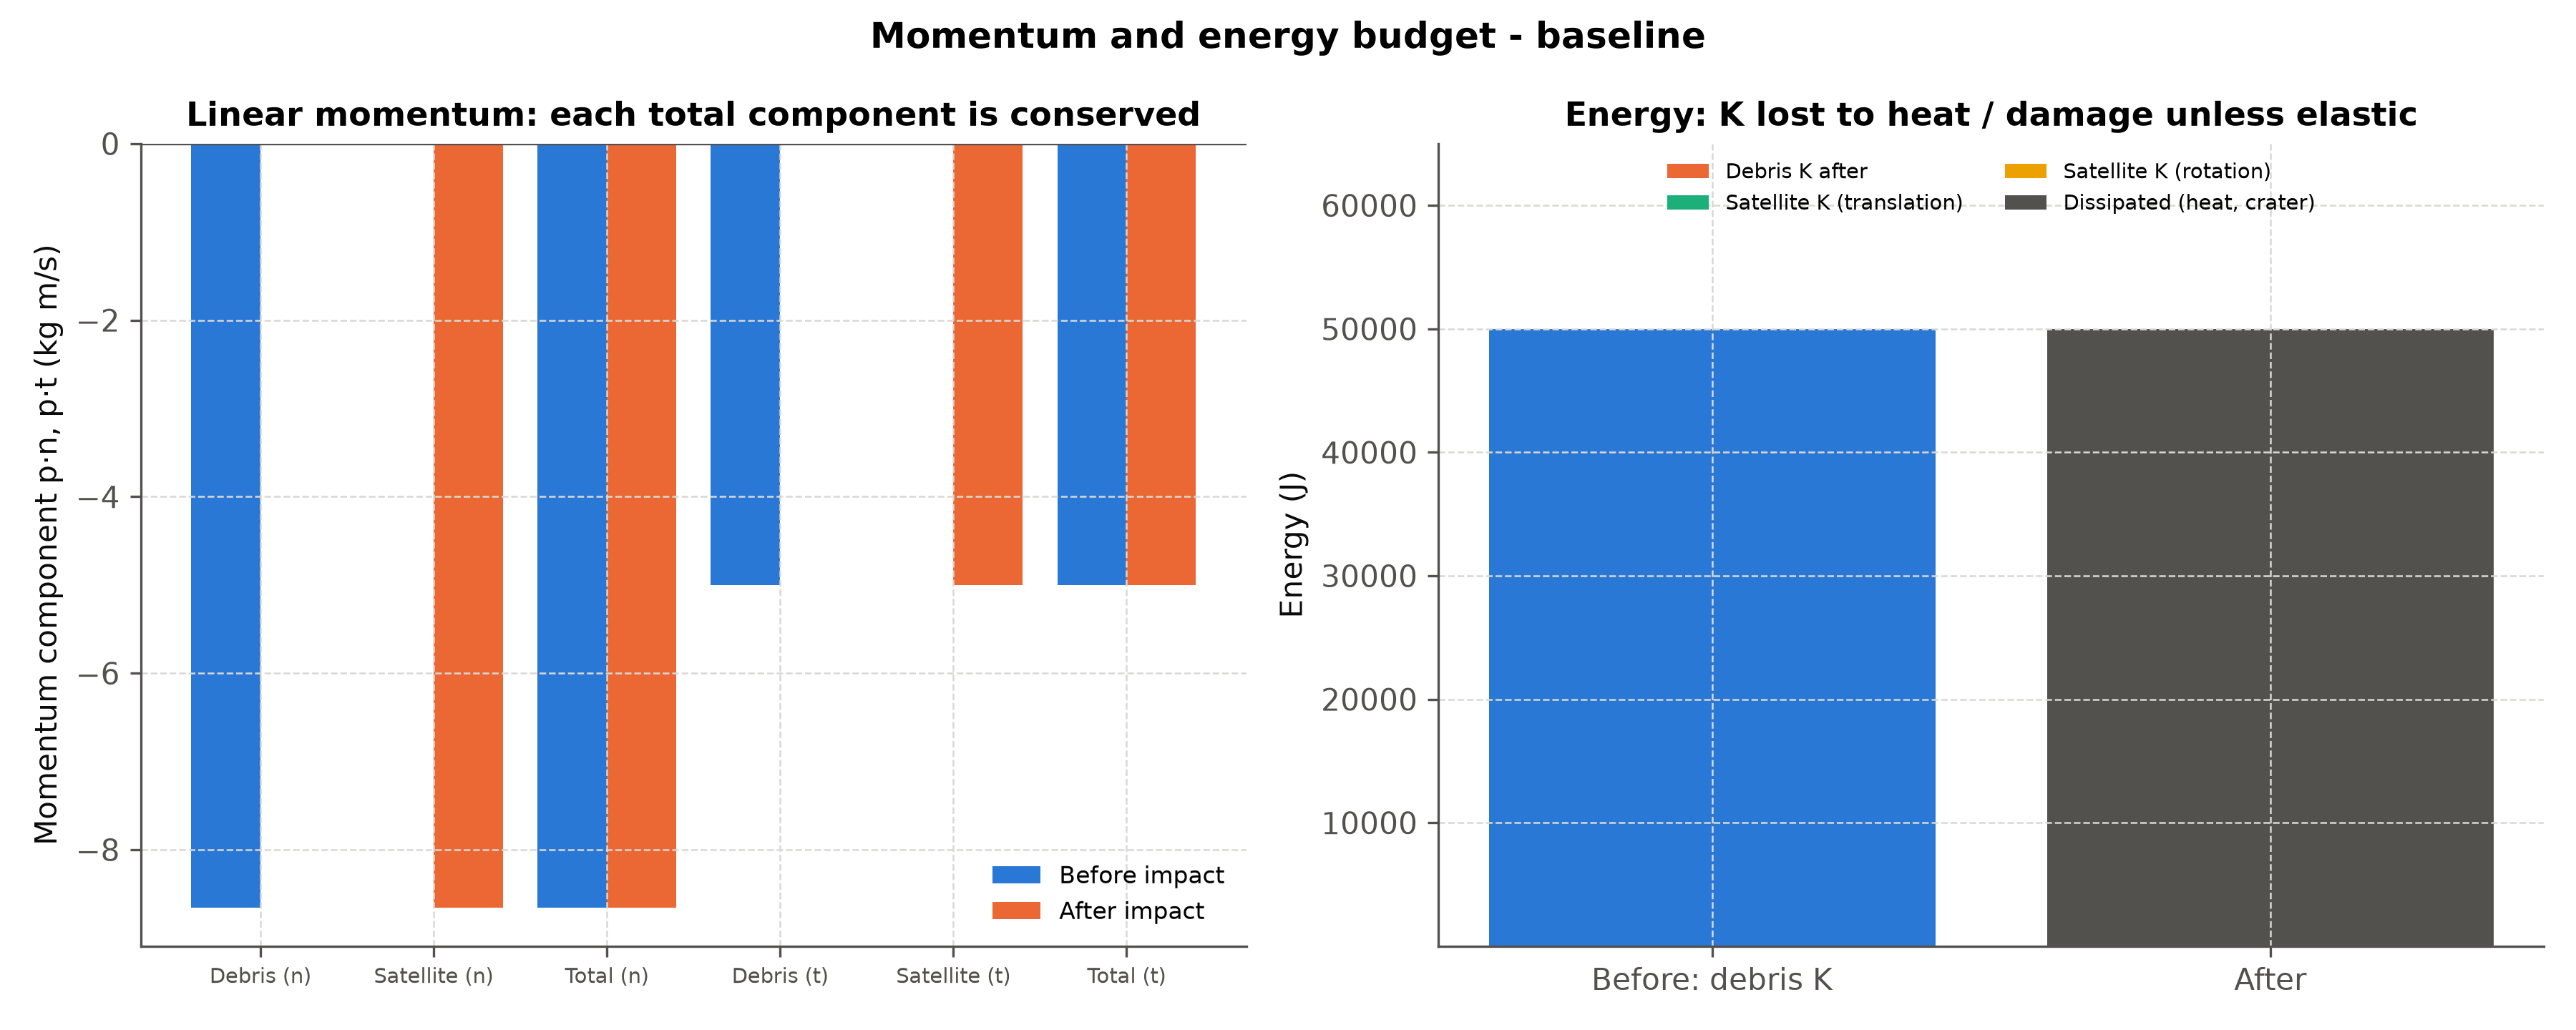
\includegraphics[width=0.5\linewidth]{image/results/budget_baseline.png}
    \caption{Baseline ($30^\circ$, completely inelastic).}
    \label{fig:budget-baseline}
  \end{subfigure}
  \begin{subfigure}{\linewidth}\centering\centering
    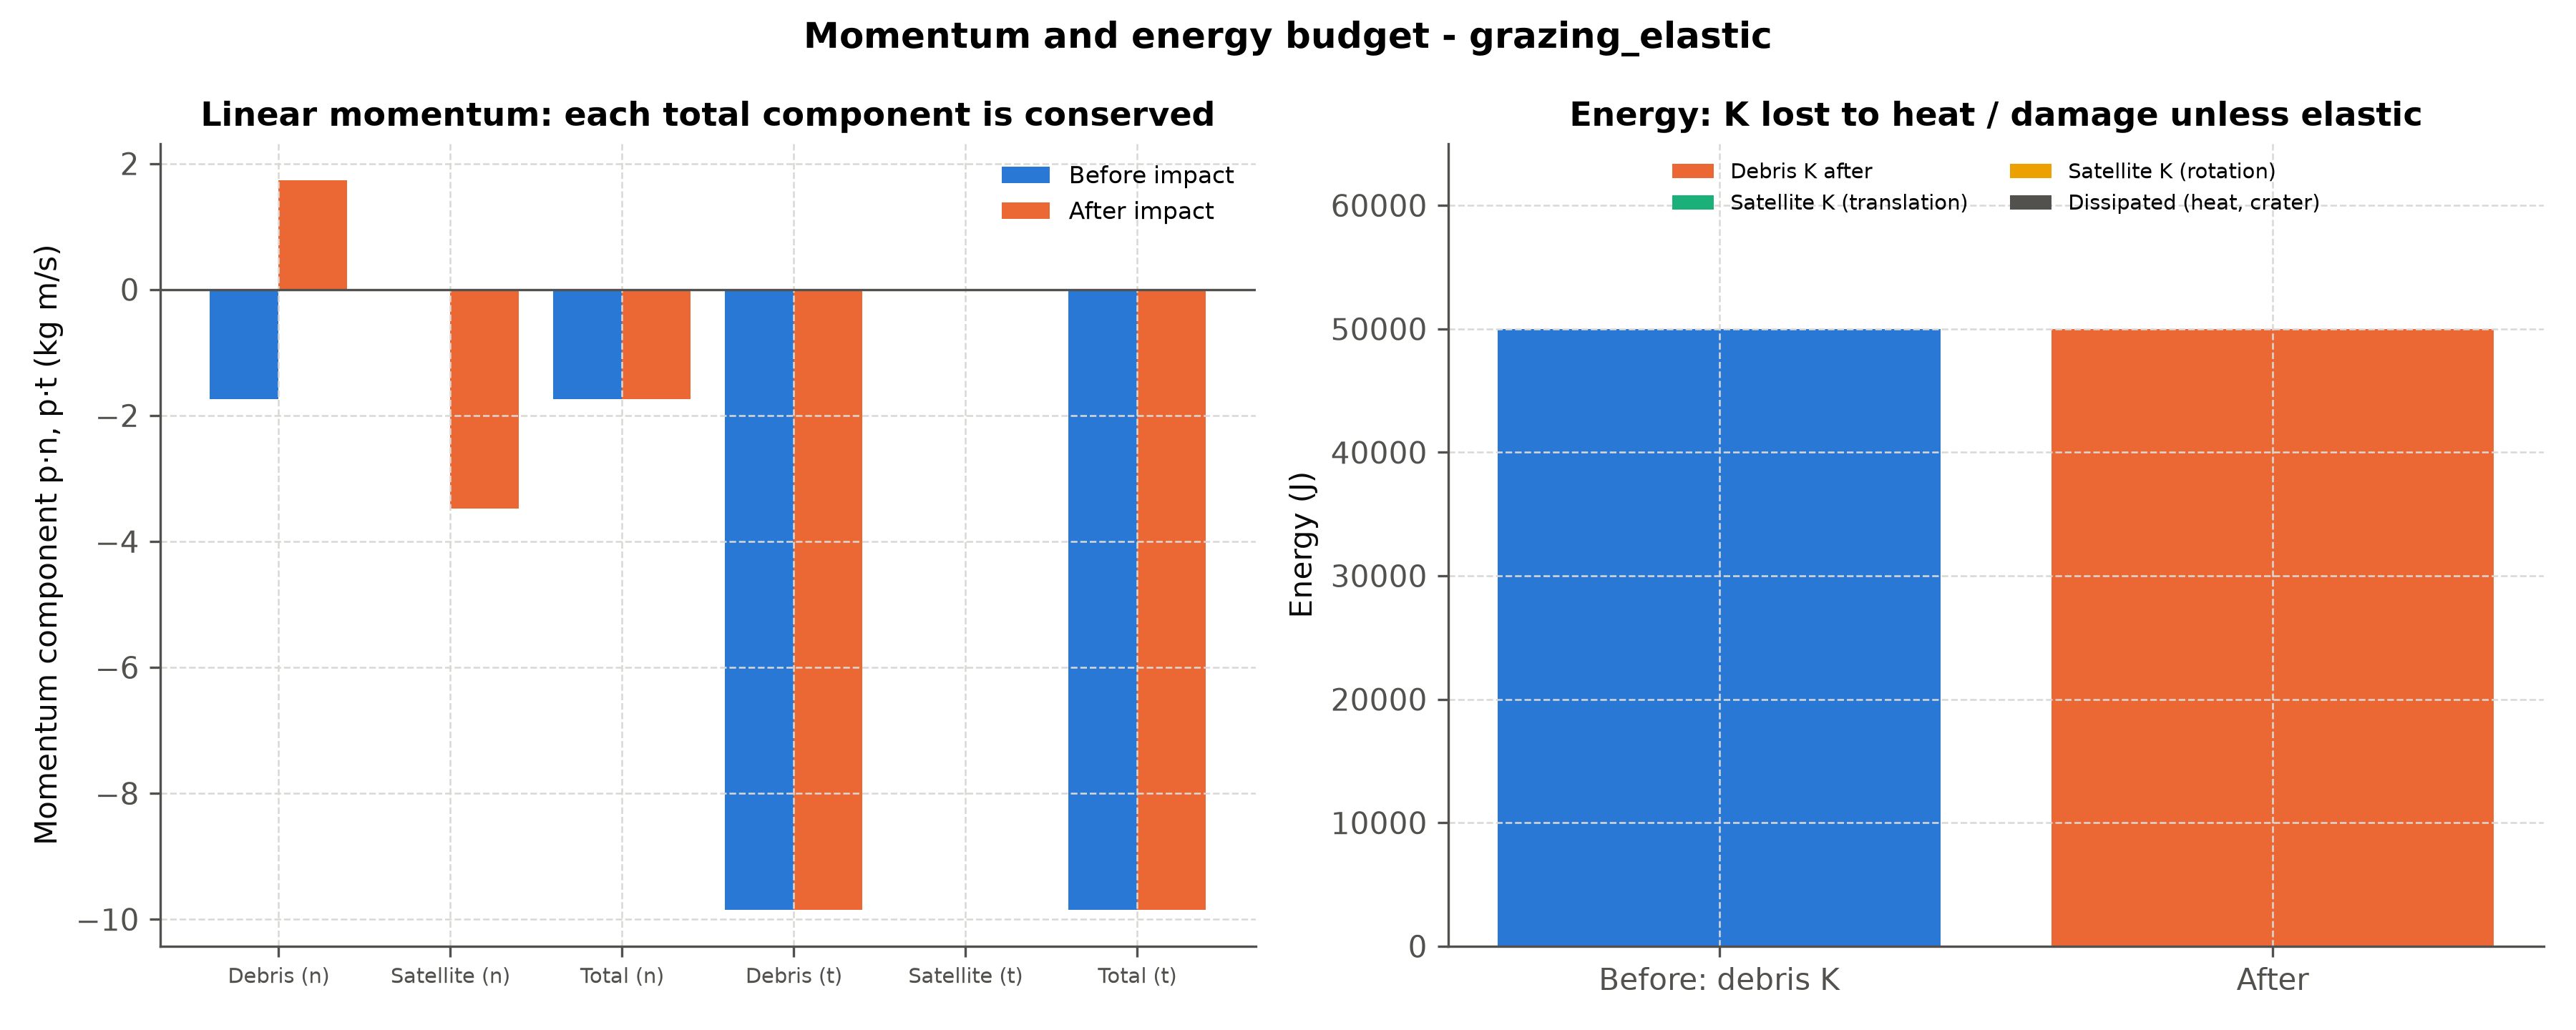
\includegraphics[width=0.5\linewidth]{image/results/budget_grazing_elastic.png}
    \caption{Grazing ($80^\circ$, elastic).}
    \label{fig:budget-grazing}
  \end{subfigure}
  \caption{Momentum components along $\hat{\vect n}$ and $\hat{\vect t}$
  (left) and energy budget (right) before and after the impact.}
  \label{fig:budget}
\end{figure}


\subsection{Parametric study}

Figure~\ref{fig:mass-speed} shows $|\Delta\vect V|$ for all 4047
mass--speed pairs with the baseline geometry. It goes from
$2.0\times10^{-6}\unit{m\,s^{-1}}$ (1~mg at $1\unit{km\,s^{-1}}$) up to
$269\unit{m\,s^{-1}}$ (10~kg at $15\unit{km\,s^{-1}}$). When $m\ll M$,
$|\Delta\vect V|\approx m v_0/M$, so it grows in direct proportion to both
mass and speed.

\begin{figure}[H]
  \centering
  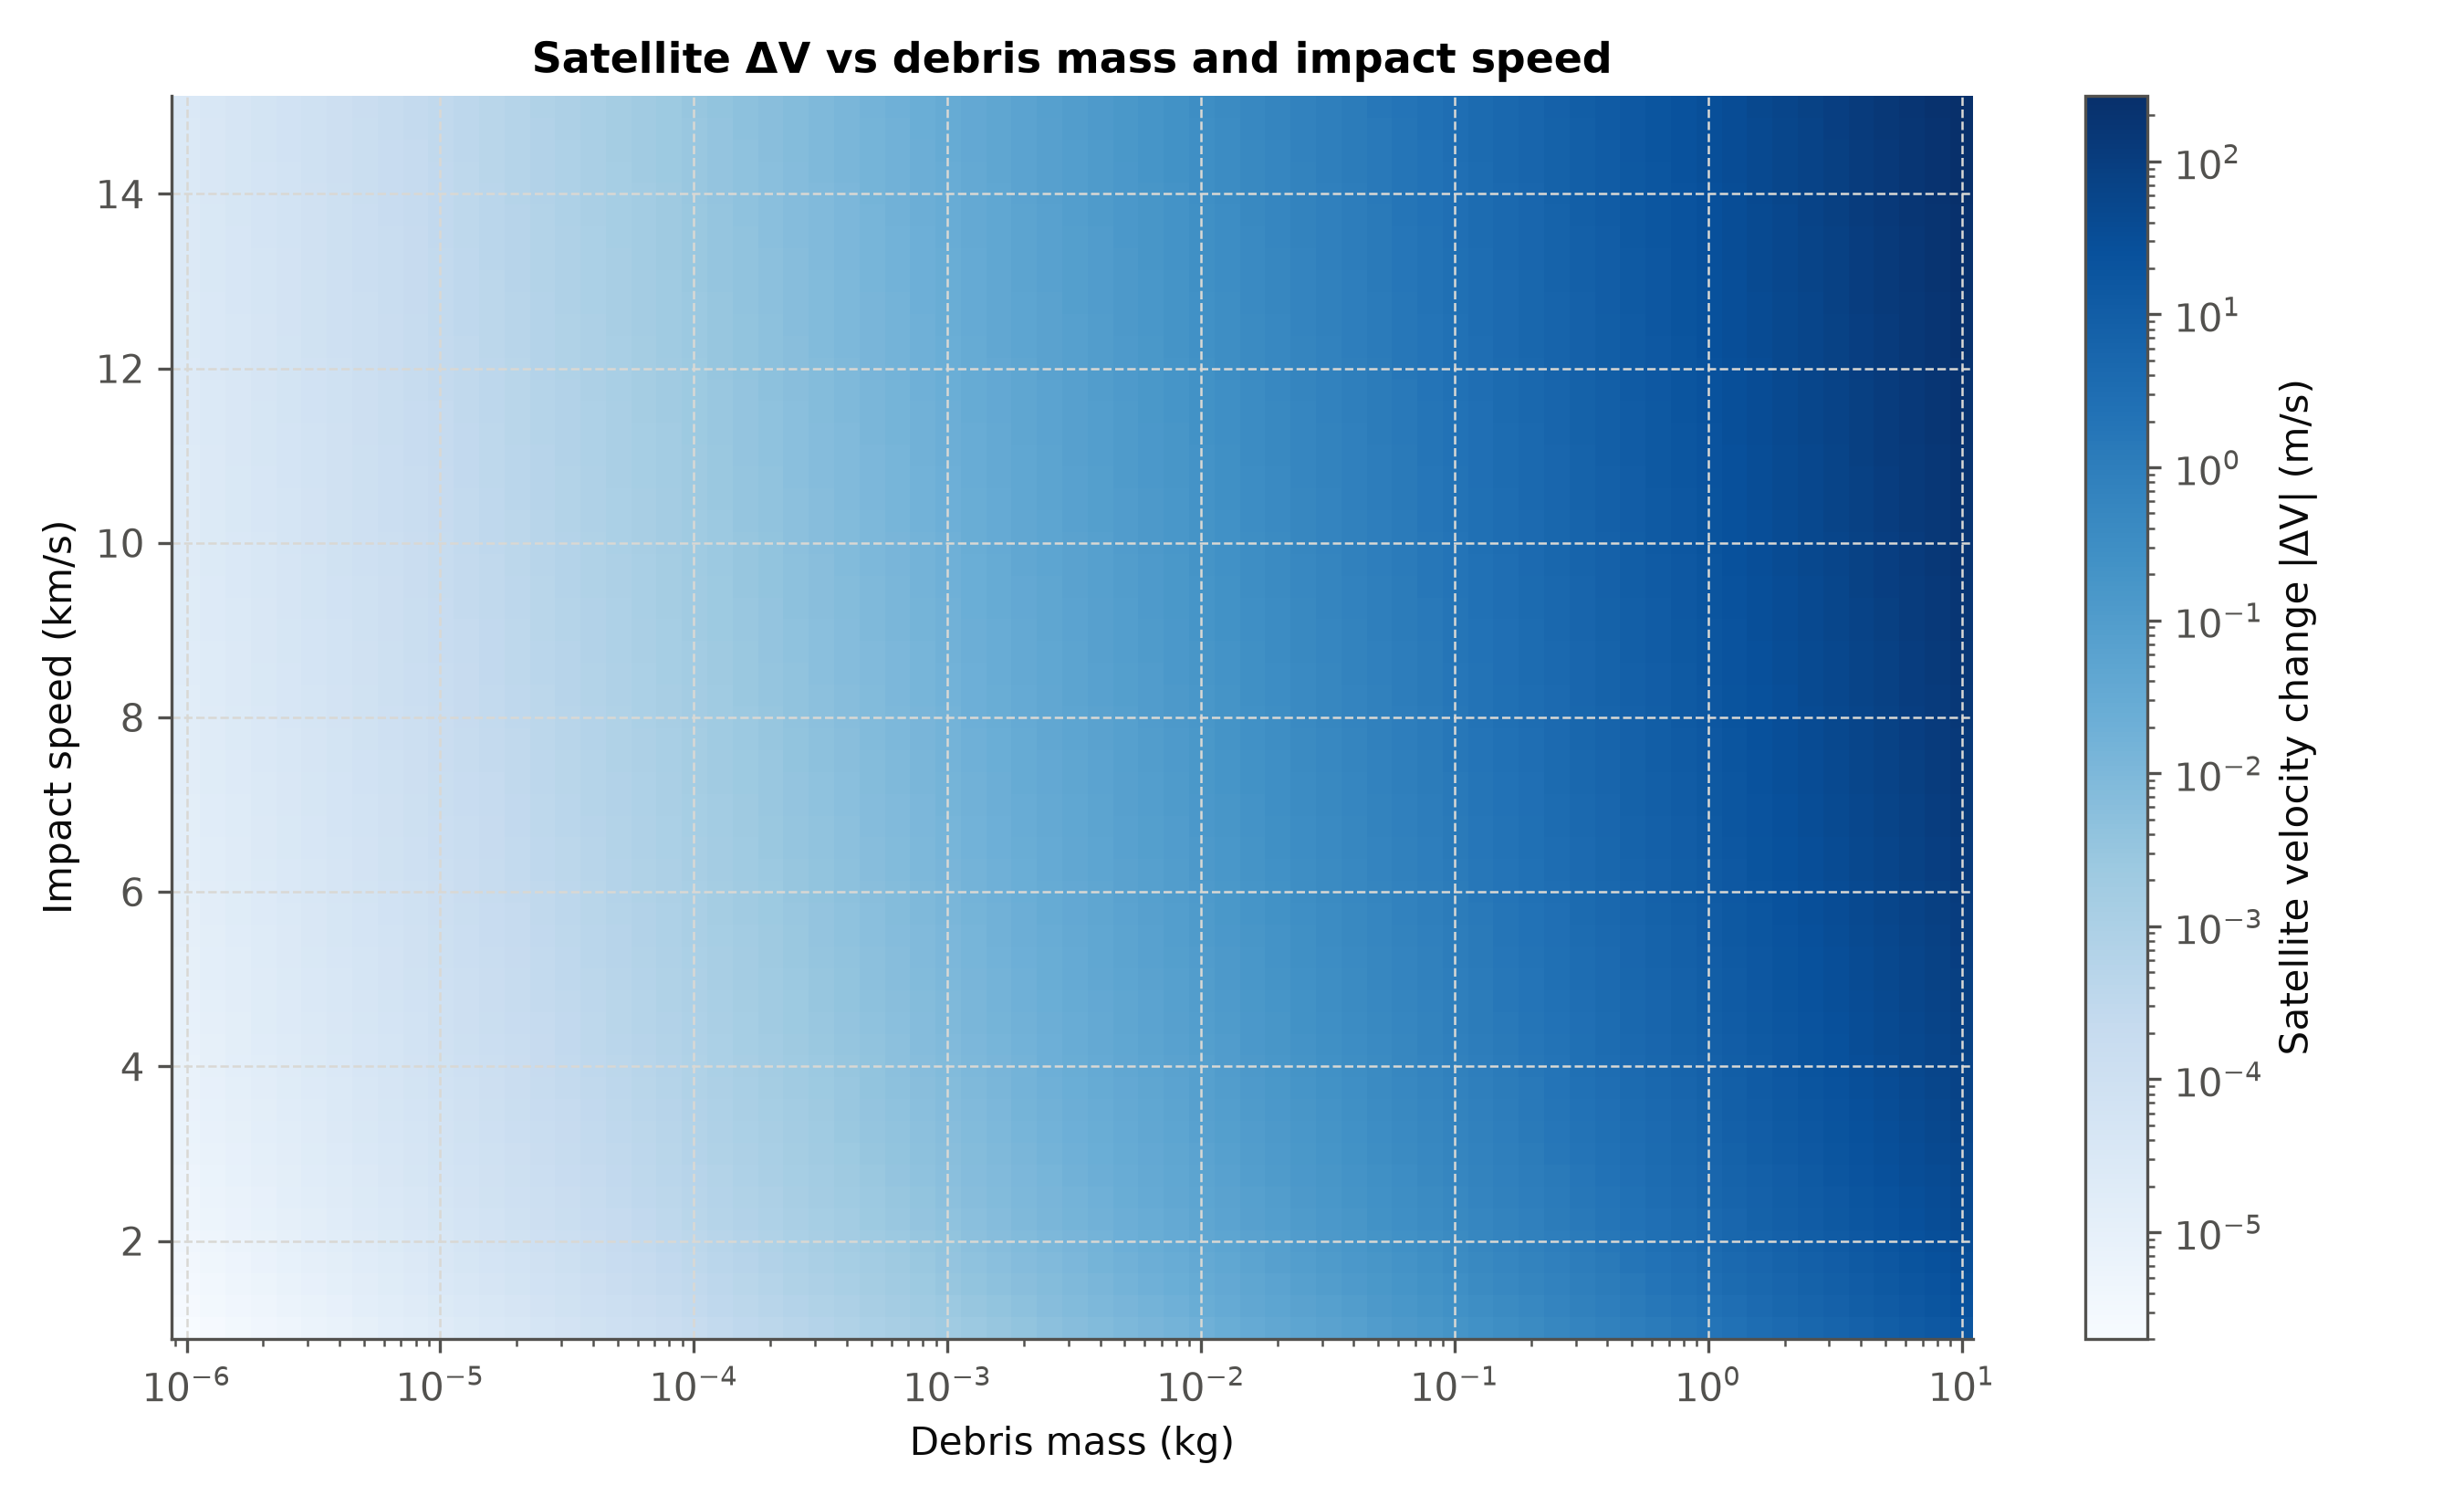
\includegraphics[width=0.38\linewidth]{image/results/01_mass_speed_dv_map.png}
  \caption{Satellite velocity change versus debris mass and impact speed
  (baseline geometry, completely inelastic; logarithmic mass axis and
  colour scale).}
  \label{fig:mass-speed}
\end{figure}

Figure~\ref{fig:angle} shows how the impact angle matters. In the
completely inelastic case $|\Delta\vect V|=20.0\unit{mm\,s^{-1}}$ at every
angle, because the satellite absorbs the whole momentum $m\vect v_{d0}$.
In the elastic case only the normal momentum is reversed, so
$|\Delta\vect V|\approx 2mv_0\cos\theta/M$ drops from $40.0$ to
$0.70\unit{mm\,s^{-1}}$. The two curves cross at $\theta=60^\circ$, where
$2\cos\theta=1$. The spin only depends on the normal part of the
velocity, because here the sideways velocity points along $\vect r$ and
gives no torque. So $|\omega|\propto\cos\theta$ in both cases, and the
elastic spin is about twice the inelastic one.

\begin{figure}[H]
  \centering
  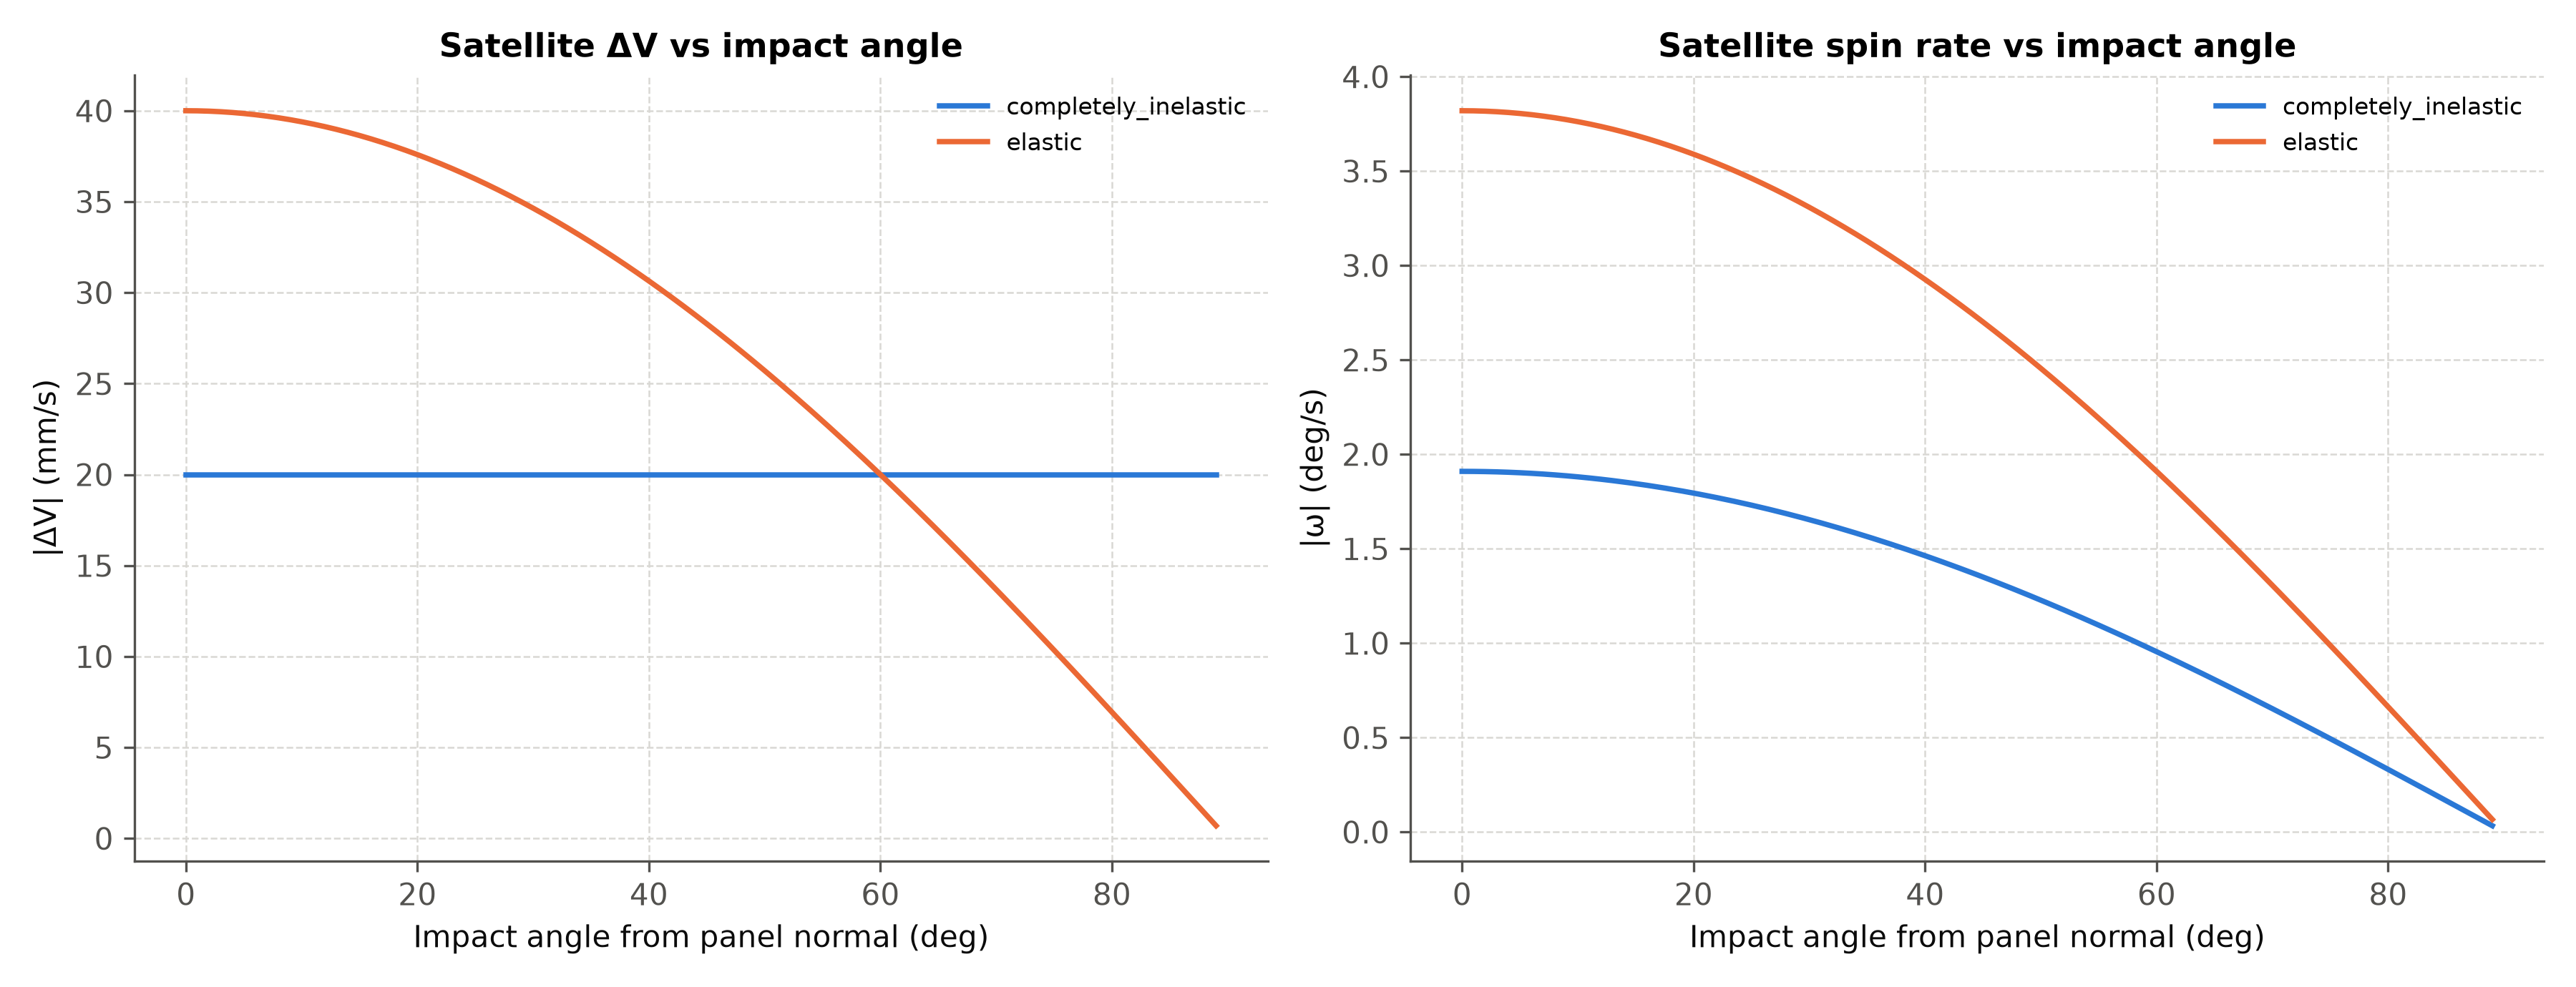
\includegraphics[width=0.5\linewidth]{image/results/02_impact_angle_sweep.png}
  \caption{Satellite velocity change (left) and spin rate (right) versus
  impact angle for both collision types (179 angles each).}
  \label{fig:angle}
\end{figure}

\begin{figure}[H]
  \centering
  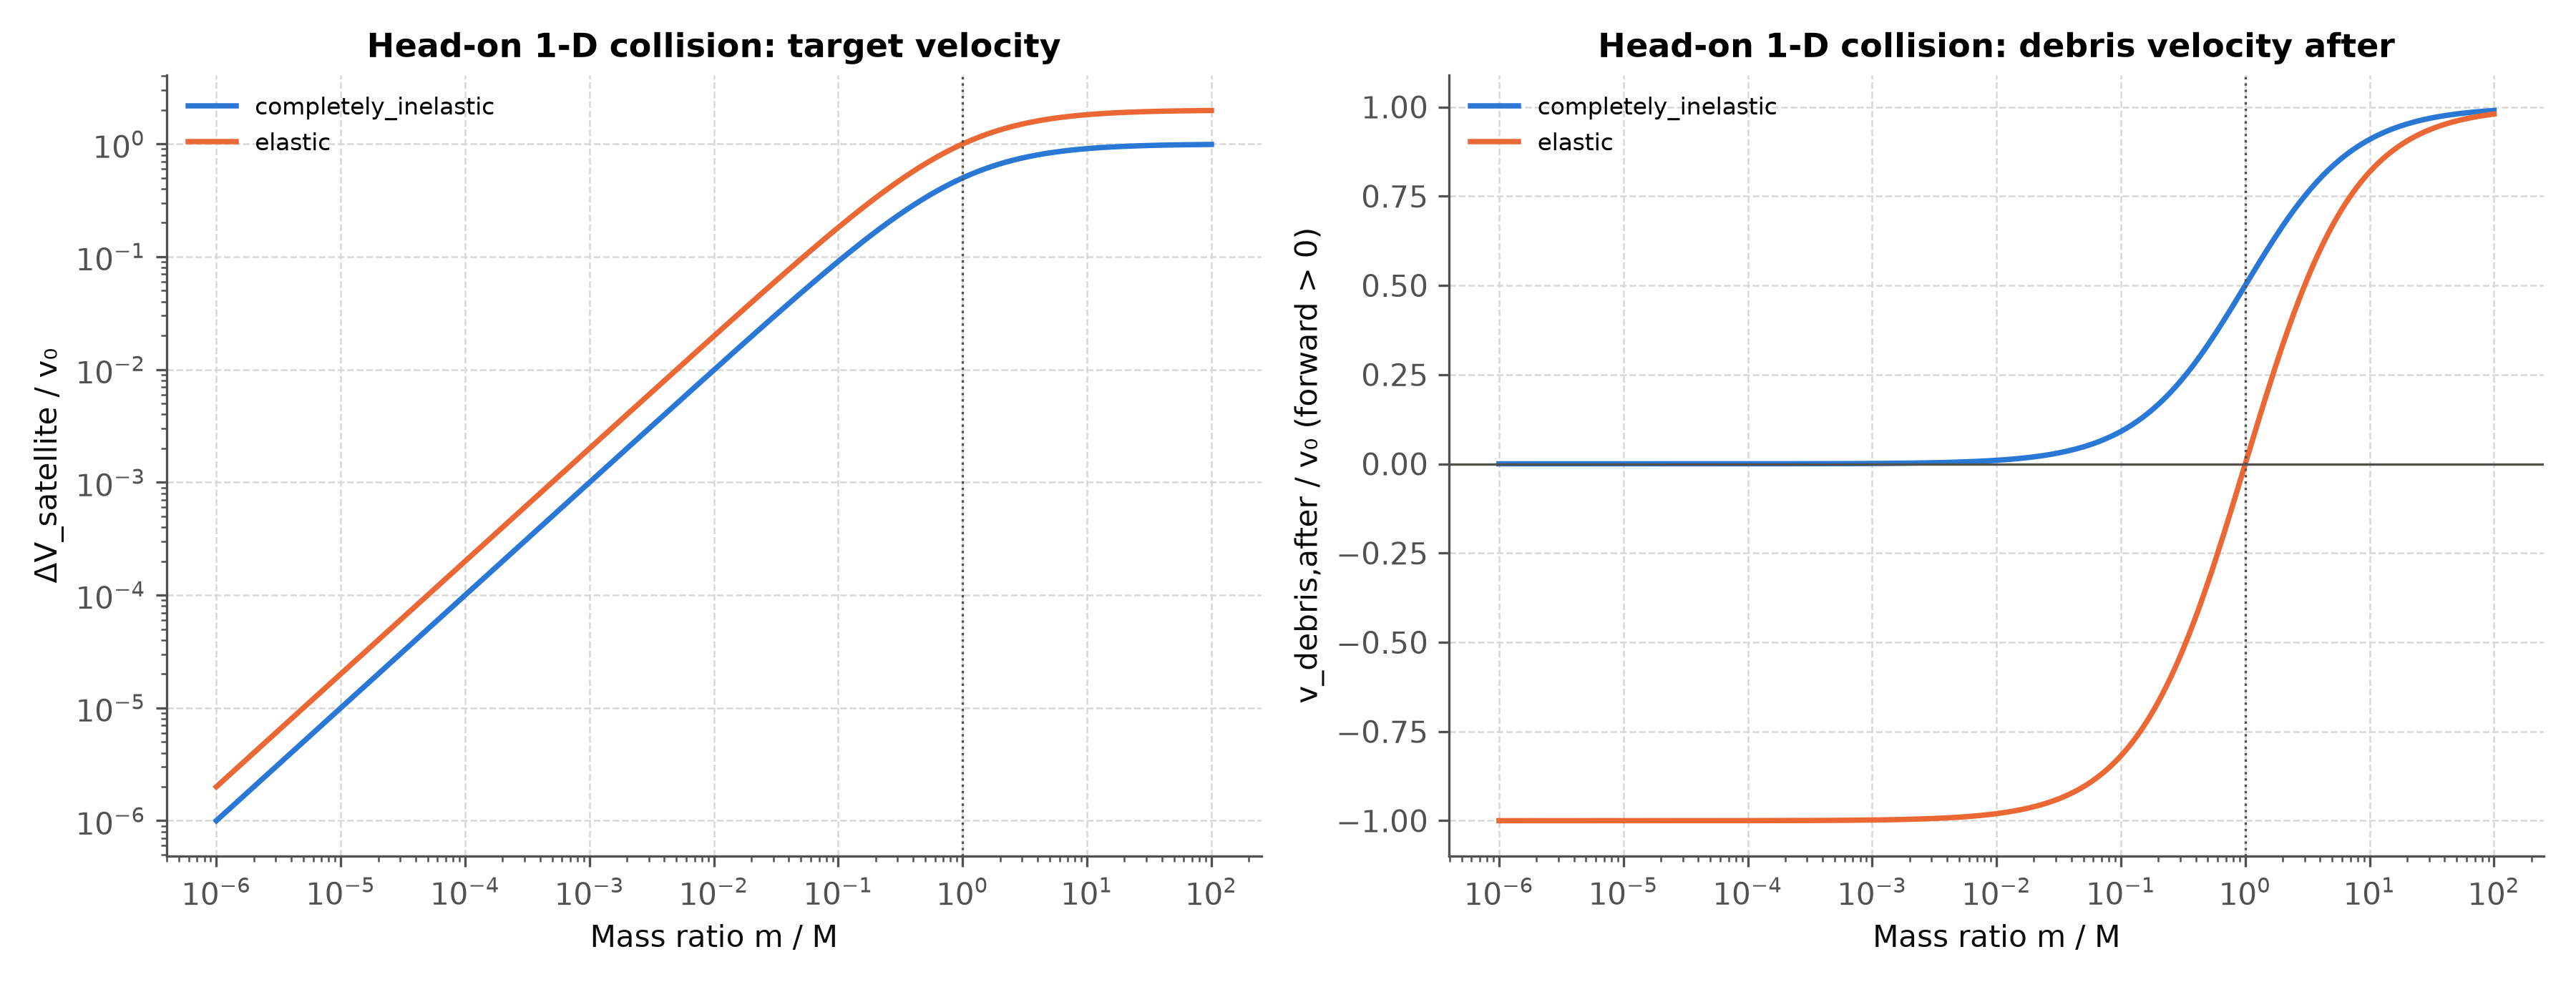
\includegraphics[width=0.5\linewidth]{image/results/03_mass_ratio_sweep.png}
  \caption{Head-on hit through the CoM: satellite velocity (left) and
  fragment velocity after the impact (right), both divided by $v_0$,
  versus the mass ratio $m/M$ (241 ratios per collision type).}
  \label{fig:mass-ratio}
\end{figure}

Figure~\ref{fig:mass-ratio} gives the familiar 1-D collision. When
$m\ll M$, the satellite's velocity grows in proportion to $m/M$ (twice as
fast in the elastic case), and in the elastic case the fragment bounces
back at $-v_0$. When $m\gg M$, the target reaches $2v_0$ (elastic) or
$v_0$ (completely inelastic). Over all 482 points, the biggest difference
from the 1-D formulas is $6.7\times10^{-16}\,v_0$.
Table~\ref{tab:extreme} lists the limiting cases.

\begin{table}[H]
  \centering\footnotesize
  \caption{Limiting cases (baseline values unless stated).}
  \label{tab:extreme}
  \begin{tabular}{@{}lrrr@{}}
    \toprule
    Case & $|\Delta\vect V|$ (m\,s$^{-1}$) & $\omega$ (rad\,s$^{-1}$) & $E_{\mathrm{diss}}/K_0$ \\
    \midrule
    1~\textmu g fragment & $2.0\times10^{-8}$ & $-2.9\times10^{-8}$ & 1.000000 \\
    $m=M$, head-on, elastic & 10\,000 & 0 & 0 \\
    $m=M$, head-on, completely inelastic & 5000 & 0 & 0.5 \\
    $m=100M$, head-on, elastic & 19\,801.98 & 0 & 0 \\
    Near-grazing, $89^\circ$ & 0.0200 & $-5.8\times10^{-4}$ & 0.999998 \\
    Hit at the CoM, $\vect r=\vect 0$ & 0.0200 & 0 & 0.999998 \\
    Baseline, elastic & 0.0346 & $-0.0577$ & 0 \\
    \bottomrule
  \end{tabular}
\end{table}
